The CANDECOMP/PARAFAC (CP) tensor decomposition is an important tool
for data analysis in applications such as chemometrics~\cite{MuStGrBr13}, biogeochemistry~\cite{JaCaYa14},
neuroscience~\cite{AcBiBiBr07,DaGiCaWa13,CoLiKuGo15}, cyber traffic analysis~\cite{MaGuFa11}, and many others.
%
We consider the problem of accelerating the alternating least squares (CP-ALS) algorithm using randomization.

Because randomized methods have been used successfully for solving
linear least squares problems~\cite{DrMaMuSa11,blendenpik,sketching}, it is natural that they might prove
beneficial to CP-ALS since its key kernel is the solution of a least
squares problem. However, the CP-ALS least squares subproblem has a
special structure that already greatly reduces its cost (see~\cref{eqn:nicegram}), so it is not obvious that sketching would be beneficial.
Nevertheless, we find that our randomized algorithms significantly reduce the memory and computational overhead of the CP-ALS process for dense tensors and moreover positively impact algorithmic robustness.
To the best of our knowledge, this is the first successful application of matrix sketching methods in the context of CP.
Our contributions are as follows:
\begin{itemize}
\item 
The least squares coefficient matrix in the CP-ALS subproblem is a Khatri-Rao product of factor matrices. 
Our randomized algorithm prefers \emph{incoherent} matrices.
We prove that the coherence of the Khatri-Rao product is bounded 
above by the product of the coherence of its factors:
\begin{lemma} \label{lem:krp}
Given $\M{A} \in \mathbb{R}^{I \times J}$ and $\M{B} \in \mathbb{R}^{K \times L}$, $\mu(\M{A} \odot \M{B}) \leq \mu(\M{A})\mu(\M{B})$.
\end{lemma}
\item We introduce the CPRAND algorithm that uses a randomized least squares solver for the subproblems in CP-ALS and never explicitly forms the full Khatri-Rao matrices used in the subproblems.
We also introduce the complementary CPRAND-MIX algorithm that employs efficient \emph{mixing} to promote incoherence and thereby improves the robustness of the method.
\item We derive a novel, lightweight stopping condition that estimates
  the model fit error, and we prove its accuracy using Chernoff-Hoeffding bounds:
  \begin{lemma} For any $\gamma \in (0,1)$, we can bound the relative
  difference in the approximated and true error as
\begin{align*}
\Pr\left\{\sqrt{1-\gamma} \leq \frac{(P \hat \mu)^{1/2}}{\|\T{E}\|} \leq \sqrt{1+\gamma}\right\} \leq \exp\left(-2\frac{\gamma^2 \mu^2 \hat P}{\mu_{\text{max}}^2}\right),\\
\end{align*}
\end{lemma}
(for details see~\cite{caseyb}).
\item We demonstrate the speed and robustness of our algorithms over a
  large number of synthetic tensors as well as real-world data
  sets. In comparison with CP-ALS, CPRAND is faster and much less sensitive to
  the starting point. (For instance, see~\cref{fig:tvsfmain} for speed and~\cref{fig:tammyexperiment} for robustness).
\end{itemize}
We give an example of our methods' fast time to solution in \cref{fig:tvsfmain},
comparing CPRAND and CPRAND-MIX with CP-ALS.
For the CPRAND methods, we use 100 sampled rows for each least squares solve.
The randomized methods converge much more quickly, in only a few
iterations. 
The fit is not monotonically increasing for the randomized methods due
to (small) variations in the solution to each randomized subproblem.
\begin{figure}[tbhp]
  \centering \subfloat[Random $300\times300\times300$ tensor]{
    \begin{tikzpicture}
      \begin{axis}[width=.49\textwidth, height=1.8in, grid=major,
        xlabel={time ($s$)}, ylabel={fit},
        xmin=0,xmax=20,ymin=0.9,ymax=1,legend style={font=\smaller},
        legend pos=south east,style={thick}
        ]
        \addplot[color=cpalsncolor,mark=*,mark size=1pt] table [x=cpt,y=cpf] {./data/tvsf300.dat};
        \addplot[color=cprandcolor,mark=*,mark size=1pt] table [x=cprandt,y=cprandf] {./data/tvsf300.dat};
        \addplot[color=cprandfcolor,mark=*,mark size=1pt] table [x=cprandfftt,y=cprandfftf] {./data/tvsf300.dat};
        \addplot[mark=none, black, samples=2,very thin,dashed] coordinates {(0,0.99) (20,0.99)};
      \end{axis}
    \end{tikzpicture}
    \label{fig:tvsf}}
  \subfloat[Random $80\times80\times80\times80$ tensor]{
    \begin{tikzpicture}
      \begin{axis}[width=.49\textwidth, height=1.8in, grid=major,
        xlabel={time ($s$)},
        xmin=0,xmax=20,ymin=0.9,ymax=1,legend style={font=\smaller},
        legend entries={CP-ALS,CPRAND,CPRAND-MIX}, legend pos=south east,style={thick}
        ]
        \addplot[color=cpalsncolor,mark size=1pt,mark=*] table [x=cpt,y=cpf] {./data/tvsf80.dat};
        \addplot[color=cprandcolor,mark size=1pt,mark=*] table [x=cprandt,y=cprandf] {./data/tvsf80.dat};
        \addplot[color=cprandfcolor,mark size=1pt,mark=*] table [x=cprandfftt,y=cprandfftf] {./data/tvsf80.dat};
        \addplot[mark=none, black, samples=2,very thin,dashed] coordinates {(0,0.99) (20,0.99)};
      \end{axis}
    \end{tikzpicture}
    \label{fig:tvsf2}}
  \caption{Runtime comparison for fitting the CP tensor decomposition
    on random synthetic tensors generated
    to have rank 5, factor collinearity of 0.9, and 1\% noise.
    We compare a single run of three methods using a target rank of 5.
    CPRAND and CPRAND-MIX use random initialization,
    100 sampled rows for each least squares solve. 
    CP-ALS uses HOSVD initialization.
    The marks indicate each iteration.
    The
    thin dashed black line represents a fit of 99\%, which is the best
    we expect when the noise is 1\%.} 
    \label{fig:tvsfmain}
  \end{figure}


\begin{figure}[h]
  \centering 
  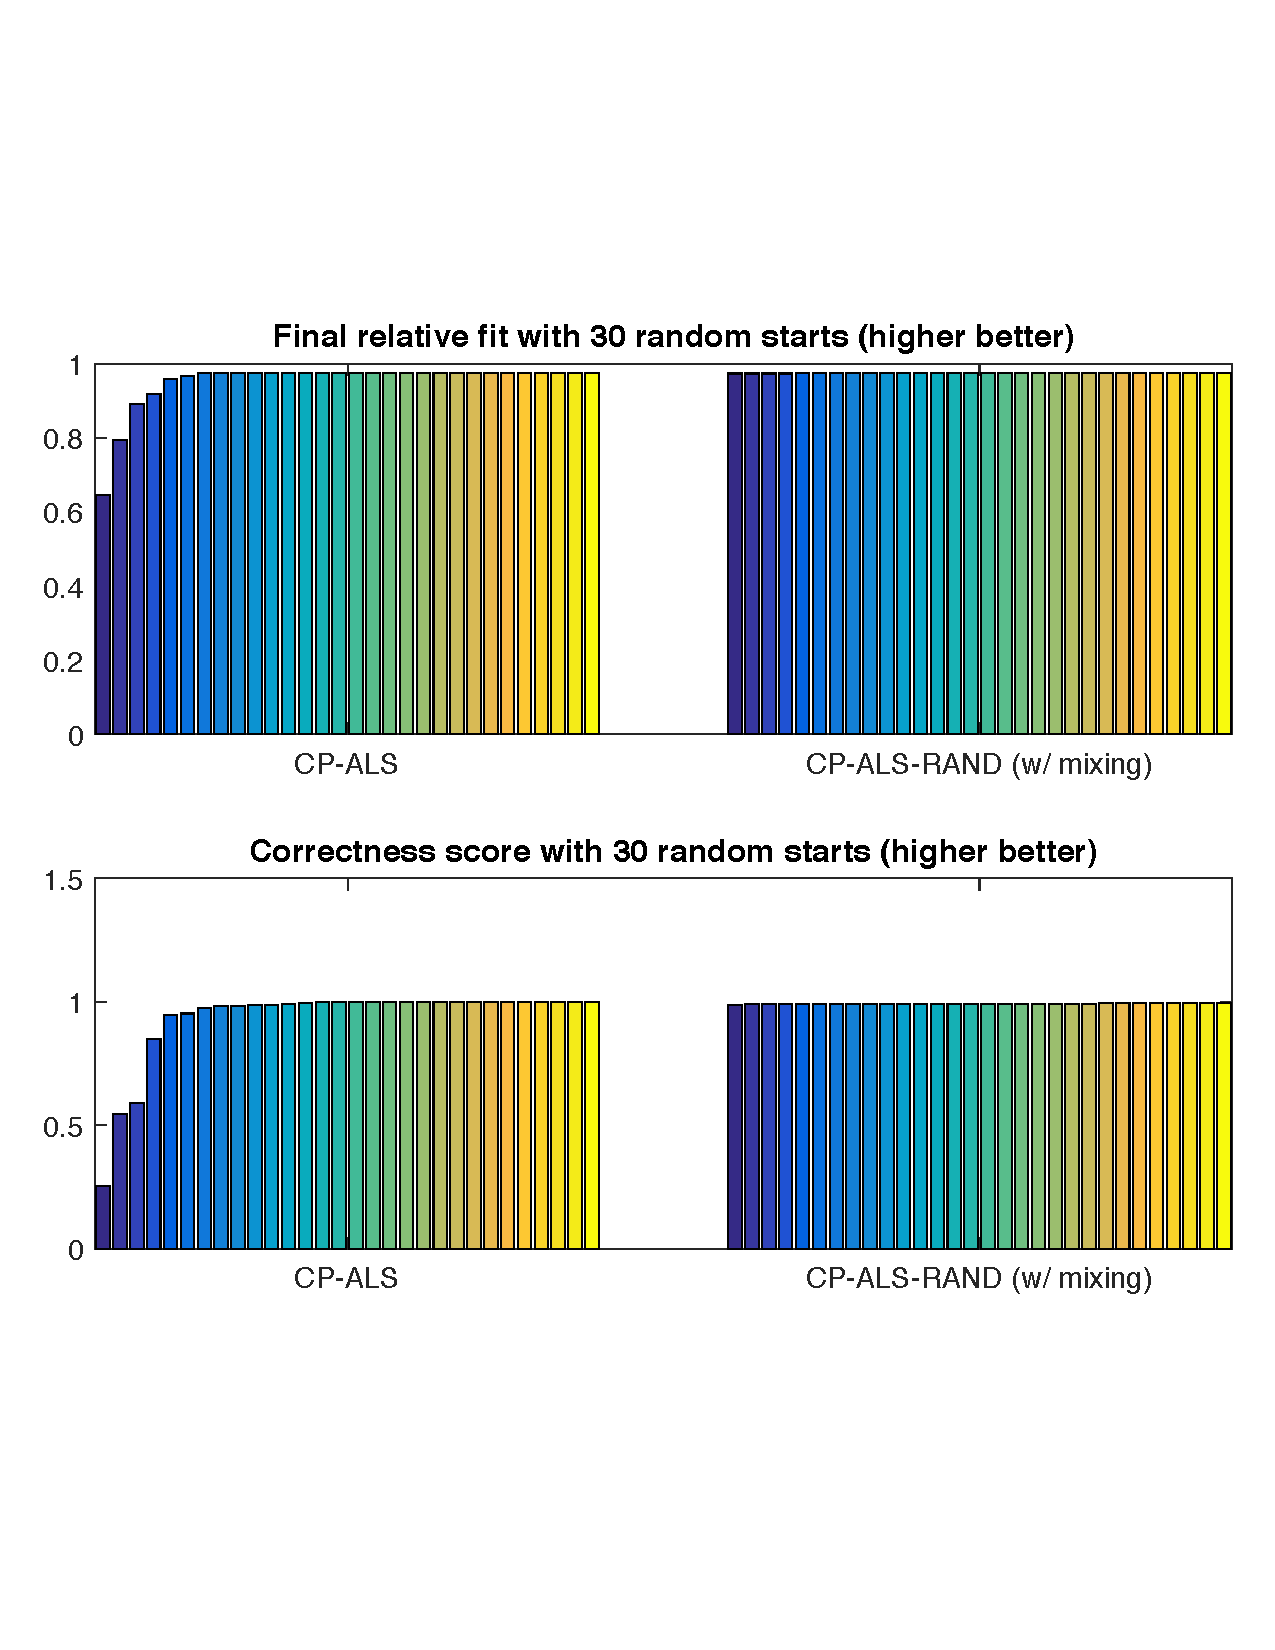
\includegraphics[width=0.6\linewidth]{figs/tammyexperiment}
  \caption{To demonstrate robustness, we show fit and score over 30 runs of a standard CP-ALS algorithm vs. our algorithm (CP-ALS-RAND with mixing) on a $5 \times 201 \times 61$ tensor drawn from chemometrics. Fit corresponds to the normalized residual error~(\cref{eqn:residual}) subtracted from 1. Score measures how well the recovered factors correspond to the best known actual factors.}
  \label{fig:tammyexperiment}
\end{figure}
